\documentclass[
  a4paper,            % DIN A4
  DIV=10,             % Schriftgröße und Satzspiegel
  oneside,            % einseitiger Druck
  BCOR=5mm,           % Bindungskorrektur
  parskip=half,       % Halber Abstand zwischen Absätzen
  numbers=noenddot,   % Kein Punkt hinter Kapitelnummern
  bibtotoc,           % Literaturverzeichnis im Inhaltsverzeichnis
  listof=totoc        % Abbildungs- und Tabellenverzeichnis im Inhaltsverzeichnis
]{scrreprt}
\usepackage{../style/thesisstyle}
\usepackage{subcaption}

\makeglossaries           % create all glossary entries (remember: run makeglossaries manually)
\loadglsentries{thesisglossaries.tex}  % load acronym, symbol and glossarie entries

\sisetup{locale = DE}     % siunitx locale setup
%\DeclareSIUnit \fps{fps}  % a custom unit (usage: \SI{24}{\fps})

\begin{document}
% !TEX root = ../thesis.tex
%
% configurations
%

% text field
%-> replace supervisor names with correct ones
\firstSupervisor{Prof. Dr.-Ing. Jane Doe}
\secondSupervisor{Prof. Dr. John Doe}

% text field
%-> replace title with your thesis title
\thesisTitle{Das Leben, das Universum und der ganze Rest}
\thesisTitleEN{Life, the Universe and Everything}

% text field
%-> replace the key words with your own key words
\keywordsDE{Leben, Universum, Alles}
\keywordsEN{Life, Universe, Everything}

% text field
%-> replace the text with a description of the thesis
\abstractDE{Arthur Dents Reise in eine neue Zukunft \dots}
\abstractEN{Arthur Dents travel to a new future \dots}

% text field
%-> replace john with your name
\thesisAuthor{John Doe}

% text field
%-> enter the submission date
\submissionDate{07. Juni 1954}

% switch - uncomment only one
%-> uncomment NDA or public
%\NDA{yes}
\NDA{no}

% switch - uncomment only one
%-> uncomment cover or cover Corporate Design 2017
\Cover{CD2017}
%\Cover{CD2017NoLogo}
%\Cover{Std2018}

% switch - uncomment only one
%-> uncomment to show list of figures or not
\ListOfFigures{yes}
%\ListOfFigures{no}

% switch - uncomment only one
%-> uncomment to show list of tables or not
\ListOfTables{yes}
%\ListOfTables{no}

% switch - uncomment only one
%-> uncomment to show list of accronyms or not
\ListOfAccronyms{yes}
%\ListOfAccronyms{no}

% switch - uncomment only one
%-> uncomment to show list of symbols or not
\ListOfSymbols{yes}
%\ListOfSymbols{no}

% switch - uncomment only one
%-> uncomment to show list of glossary entries or not
\Glossary{yes}
%\Glossary{no}

% switch - uncomment only one
%-> uncomment the study course you are in
\studycourse{ITS}
%\studycourse{TI}
%\studycourse{AI}
%\studycourse{WI}
% \studycourse{EI}
%\studycourse{REE}
%\studycourse{BMT}
%\studycourse{BMT-st}    % Study / home assignment in BMT
%\studycourse{MAI}
%\studycourse{MIK}
%\studycourse{MA}
    % load all settings

\hyphenation{Ba-che-lor-the-sis Mas-ter-the-sis}

% Cover page here, no page number
\ICoverPage

% PDF Metadata
% !TEX root = ../thesis.tex
%
% PDF Metadata integration
% @author Thomas Lehmann
%

% PDF Metadata
\hypersetup{
pdftitle={\IthesisTitle},
pdfauthor={\IthesisAuthor},
pdfkeywords={\IkeyWordsEN}
}

% Titlepage is page one even if the number is not shown.
\pagenumbering{roman}
% Title page here
% !TEX root = ../thesis.tex
%
% title page
% @author Thomas Lehmann
% Hints for title page and page numbering: https://en.wikipedia.org/wiki/Title_page
%
\title{\IthesisTitle}   % set latex default title to be used by hyperref in pdf
\author{\IthesisAuthor} % set latex default author to be used by hyperref in pdf

\newpage
\thispagestyle{empty}
{\fontfamily{phv}\selectfont
  \hfuzz=20pt       % suppress warnings due to extenstion onto page margins

  % Author of thesis
  \vspace*{1cm}
  \begin{minipage}[b]{\textwidth}
    \fontsize{14pt}{20pt}
    \selectfont
    \begin{center}
      \IthesisAuthor
    \end{center}
  \end{minipage}

  % Title of thesis
  \vspace{1.5cm}
  \begin{minipage}[b][0cm][t]{\textwidth}
    \fontsize{18pt}{20pt}
    \selectfont
    \begin{center}
      \IthesisTitle
    \end{center}
  \end{minipage}

  % Important information
  \begin{textblock*}{\textwidth}(40mm,210mm)
    \begin{minipage}[b]{\textwidth}
      \hbadness=10001    % suppress underfull warning due to short text
      \fontfamily{cmr}\selectfont
      \fontsize{12pt}{14pt}
      \selectfont
      \IthesisKindDE ~eingereicht im Rahmen der \IthesisExaminationDE \\
      im Studiengang \textit{\IstudyCourseName} \\
      am \IthesisDepartmentFull \\
      der Fakultät Technik und Informatik\\
      der Hochschule für Angewandte Wissenschaften Hamburg\\

      Betreuender Prüfer: \IfirstSv \\
      % Zweitgutachter: \IsecondSv \\

      Eingereicht am: \ISubDate \\
    \end{minipage}
  \end{textblock*}
}


% Abstract page here
% !TEX root = ../thesis.tex
%
% abstract page
% @author Thomas Lehmann
%
\newpage
\thispagestyle{plain}
\clearpage
\hfuzz=12pt       % suppress warnings due to extenstion onto page margins

\textbf{\IthesisAuthor}

\vspace{0.3cm}
\textbf{Thema der Arbeit}

\IthesisTitle

\vspace{0.3cm}
\textbf{Stichworte}

\IkeyWordsDE

\vspace{0.3cm}
\textbf{Kurzzusammenfassung}

\begin{minipage}{\textwidth}
\IabstractDE
\end{minipage}

\vspace{1.0cm}
\textbf{\IthesisAuthor}

\vspace{0.3cm}
\textbf{Title of Thesis}

\IthesisTitleEN

\vspace{0.3cm}
\textbf{Keywords}

\begin{minipage}{\textwidth}
\IkeyWordsEN
\end{minipage}

\vspace{0.3cm}
\textbf{Abstract}

\IabstractEN


% Table of contents here
\tableofcontents

% List of figures here
\IListOfFigures

% List of tables here
\IListOfTables

% List of accronyms here
\IListOfAccronyms

% List of symbols here
\IListOfSymbols

% Uncomment if list of source code is needed (rarely).
%\lstlistoflistings  % requires package listings, needs to uncommenting of usepackage

% path to the chapters folder is set to find the images used there
\graphicspath{ {./chapters/} }

% Chapters
\clearpage
\pagenumbering{arabic}
% Anforderungsanalyse
% @author Tristan Ropers
%
\chapter{Einleitung}

In dieser Ausarbeitung geht es um die Umsetzung eines Algorithmus zum gegenseitigen Ausschlusses in einem
verteilten System von Schweißrobotern. Das Problem des wechselseitigen Ausschlusses 
ist ein weit verbreitetes Problem der Informatik. In diesem konkreten Fall sollen mehrere Schweißroboter
auf eine Ressource zugreifen können und dort einen Schweißpunkt setzen, was eine Regelung der Reihenfolge
erfordert, da die Roboter nicht alle gleichzeitig auf die gegebene Ressource zugreifen können. Um diese Reihenfolge
festzulegen wird Lamports Algorithmus \citep{lamport} zum gegenseitigen Ausschluss in verteilten Systemen umgesetzt
und für diesen Anwendungsfall evaluiert.

\section{Anforderungsanalyse}

\subsection{Requirements}

In der Aufgabenstellung sind Anforderungen an die RPC-Architektur formuliert.
Zunächst werden diese analysiert und hier zusammengefasst.
Die Anforderungen umfassen die Transparenzziele, Skalierung \cite{tanenbaumvansteen}) sowie Anforderungen
an die Umsetzung und Architektur.\\
Es wurde ein hoher Grad an Transparenz gefordert.
Die Transparenzziele umfassen die Access-Transparency, Location-Transparency, Relocation-Transparency,
Migration-Transparency, Replication-Transparency, Concurrency-Transparency und Failure-Transparency \citep{tanenbaumvansteen}.
Die Skalierung beschränkt sich administrativ auf einen Administrator, der auch gleichzeitig
Benutzer des Systems ist sowie geographisch auf einen Rechner, auf dem alle Nodes 
\citep{tanenbaumvansteen} über das Loopback-Interface der Netzwerkkarte miteinander kommunizieren.
Somit entfällt die Concurrency-Transparency, da nur ein Nutzer am System beteiligt ist sowie die
Location-Transparency, Relocation- und Migration-Transparency, da alle Nodes über das Loopback-Interface
kommunizieren, welches auf eine Netzwerkkarte beschränkt ist. Die Replication-Transparency ist in diesem Zusammenhang 
uninteressant, da jede Node im System eindeutig identifizierbar ist,was Replikationen der Nodes für die Funktionsweise 
der verwendeten Algorithmen ausschließt.\\\\
Desweiteren ist ein Minimalset an Funktionen an die RPC-Architektur gefordert:

\begin{itemize}
 \item void register(int id)
 \item void welding()
 \item void setStatus(int status)
\end{itemize}

Es soll kein zentrales System, bis auf Erfassung von Daten zu Experimentabläufen, am Gesamtsystem beteiligt
sein.
Alle beteiligten Nodes (Roboter) sollen sich auf einen Zyklus einigen, in dem immer drei Roboter nacheinander
(Reihenfolge durch Lamport) schweißen.
Insgesamt soll kein Roboter mehr als drei Schweißpuntke mehr als ein anderer gesetzt haben.
Alle Roboter sollen am Ende eines Experiemntablaufs mindestens 20 Schweißpunkte gesetzt haben.
In 99\% soll ein Roboter nach einem Schweißvorgang weiterhin betriebsbereit sein. Im Umkehrschluss
ist ein Roboter in 1\% der Fälle nach einem Schweißvorgang nicht mehr betriebsbereit.\\
Zur Auswertung und Beobachtung des Ablaufs soll jeder Roboter seinen Ablauf loggen.
Daraus ergeben sich folgende Anforderungen:

\begin{table}[h!]
\begin{center}
\begin{tabular}{ |p{2.5cm}|p{11cm}| } 
 \hline
 Requirement & Registrierung eines Nodes im System \\
 \hline
 Beschreibung & Ein Node kann sich im System mit allen anderen Nodes bekannt machen. \\
 \hline
 Eingaben & id: int; eindeutige ID für den Node \\
 \hline
 Ziel & Die Node hat sich mit allen anderen im System bekanntgemacht. \\
 \hline
 Vorbedingung & Die Node ist hochgefahren und betriebsbereit. \\
 \hline
 Nachbedingung & Die Node kennt alle anderen Nodes im System und alle anderen Nodes kennen die sich 
 registrierende Node. \\
 \hline
\end{tabular}
\caption{Requirement Registrierung}
\label{table:reqregister}
\end{center}
\end{table}

\begin{table}[h!]
\begin{center}
\begin{tabular}{ |p{2.5cm}|p{11cm}| } 
 \hline
 Requirement & Ein Roboter versucht zu schweißen \\
 \hline
 Beschreibung & Ein Roboter einer Node möchte Zugriff auf die Ressource haben und einen Schweißauftrag
 ausführen. Sobald die Ressource verfügbar ist, soll der Roboter seinen Schweißauftrag ausführen.\\
 \hline
 Eingaben & / \\
 \hline
 Ziel & Der Roboter hat einen Schweißvorgang durchgeführt. \\
 \hline
 Vorbedingung & Die Node sowie der Roboter der Node ist hochgefahren und betriebsbereit. \\
 \hline
 Nachbedingung & Der Roboter hat einen Schweißvorgang abgeschlossen und geht entweder in einen Fehlerzustand
 (in 1\% der Fälle) oder bleibt betriebsbereit. \\
 \hline
\end{tabular}
\caption{Requirement Schweißen (Welding)}
\label{table:reqwelding}
\end{center}
\end{table}

\begin{table}[h!]
\begin{center}
\begin{tabular}{ |p{2.5cm}|p{11cm}| } 
 \hline
 Requirement & Bestimmung eines Zyklus \\
 \hline
 Beschreibung & Es muss sichergestellt sein, dass immer genau drei Roboter pro Zyklus einen
 Schweißauftrag ausführen. \\
 \hline
 Eingaben & / \\
 \hline
 Ziel & Ein Zyklus wird bestimmt und drei Roboter können schweißen. \\
 \hline
 Vorbedingung & Alle am Experiment teilnehmenden Nodes sowie dazugehörige Roboter sind
 hochgefahren und betriebsbereit. \\
 \hline
 Nachbedingung & Ein Zyklus wurde bestimmt und drei Nodes haben den Schweißauftrag erhalten. \\
 \hline
\end{tabular}
\caption{Requirement Bestimmung eines Zyklus}
\label{table:reqchoosecycle}
\end{center}
\end{table}

\begin{table}[h!]
\begin{center}
\begin{tabular}{ |p{2.5cm}|p{11cm}| } 
 \hline
 Requirement & Logging der Prozessabläufe \\
 \hline
 Beschreibung & Jede Node muss seinen Zustand und die Abläufe loggen. \\
 \hline
 Eingaben & logText: String; Event oder Zustand \\
 \hline
 Ziel & Ein Event oder Zustand des Nodes wurde geloggt. \\
 \hline
 Vorbedingung & Die Node sowie der Roboter der Node ist hochgefahren und betriebsbereit. \\
 \hline
 Nachbedingung & Der Zustand der Node oder das Event wurden erfolgreich geloggt. \\
 \hline
\end{tabular}
\caption{Requirement Logging}
\label{table:reqlogging}
\end{center}
\end{table}

\begin{table}[h!]
\begin{center}
\begin{tabular}{ |p{2.5cm}|p{11cm}| } 
 \hline
 Requirement & Austauschbarkeit des Algorithmus \\
 \hline
 Beschreibung & Der Algorithmus für den gegenseitigen verteilten Ausschluss soll austauschbar als Bibliothek
 in die Architektur eingebunden werden.\\
 \hline
\end{tabular}
\caption{Requirement Austauschbarkeit des Algorithmus}
\label{table:reqmutexexchangable}
\end{center}
\end{table}

\begin{table}[h!]
\begin{center}
\begin{tabular}{ |p{2.5cm}|p{11cm}| } 
 \hline
 Requirement & Randbedingungen des Prozessablaufs \\
 \hline
 Beschreibung &
 \begin{itemize}
  \item Nach dem Ablauf des Experiments sollen alle Roboter mindestens 20 Schweißpunkte
  gesetzt haben oder sich in einem Fehlerzustand befinden.
  \item Kein Roboter darf mehr als drei Schweißpunkte als ein anderer gesetzt haben.
  \item Die Anzahl der teilnehmenden Nodes (Roboter) liegt zwischen drei und 16.
 \end{itemize} \\
 \hline
\end{tabular}
\caption{Requirement Prozessbedingungen}
\label{table:reqprocess}
\end{center}
\end{table}

\clearpage

\subsection{UseCase}
\begin{table}[h!]
\begin{center}
\begin{tabular}{ |p{2.8cm}|p{11cm}| } 
 \hline
 UseCase & Prozessablauf mit mindestens drei Robotern \\
 \hline
 ID & UC01 \\
 \hline
 Beschreibung & Dieser UseCase schildert einen Prozessablauf von mindestens drei Robotern, wie
 er im Experiment durchgeführt wurde. \\
 \hline
 Vorbedingungen & Mindestens drei Roboter und der Logger werden hochgefahren.\\
 \hline
 Hauptszenario & 
 \begin{enumerate}
  \item Alle Roboter registrieren sich gegenseitig.
  \item Ein Zyklus wird bestimmt.
  \item Alle Roboter, welche im Zyklus ausgewählt wurden,\newline schweißen nacheinander.
  \item Ein neuer Zyklus wird bestimmt.
  \item Wiederholen ab Punkt 2.
 \end{enumerate} \\
 \hline
 Alternative\newline Szenarien &
 A1: \newline
 \begin{enumerate}
  \setcounter{enumi}{3}
  \item Mindestens ein Roboter ist in den Fehlerzustand gewechselt.
  \item Versuch neuen Zyklus zu bestimmen und zu schweißen.
 \end{enumerate}  \\
 \hline
 Fehlerszenarien & 
 E1: \newline
 \begin{enumerate}
   \setcounter{enumi}{2}
   \item Schweißaufträge im Zyklus können nicht abgeschlossen werden.
   \item System geht in Fehlerzustand.
 \end{enumerate} \\
 \hline
 Nachbedingung & Alle Roboter haben mindestens 20 Schweißpunkte gesetzt oder sind in einem Fehlerzustand. \\
 \hline
 Ergebnis & Das Experiment wurde erfolgreich beendet und alles wurde geloggt. \\ 
 \hline
\end{tabular}
\caption{UseCase Prozessablauf mit mindestens drei Robotern}
\label{table:usecase1}
\end{center}
\end{table}

% Design & Architektur
% @author Tristan Ropers
%
\chapter{Design \& Architektur}

Zur Umsetzung der Anforderungen wurde eine RPC-Architektur entwickelt, die es ermöglicht den Prozess
abzubilden. Im folgenden Kapitel wird diese Architektur vorgestellt sowie ihre Besonderheiten.

\section{Systemkontext}

\includenamedimage[0.9]{../diagrams/1_systemkontext.png} {Systemkontext}

Der Systemkontext des Gesamtsystems umfasst den Nutzer, welcher gleichzeitig Administrator ist und das
Gesamtsystem. Der Nutzer konfiguriert das System und startet im Anschluss die zuvor
konfigurierte Konfiguration.
\clearpage

\section{Lösungsstrategie}

Das System besteht aus einer RPC-Architektur und einer Robotersimulation. Die RPC-Architektur ermöglicht
die Kommunikation und Steuerung der Abläufe der Roboter untereinander und dient damit als Basis der
Architektur. Alle Nodes laufen auf einem Rechner, laufen also jeder auf einem Port.
Um den Bereich abzustecken, in dem die Nodes laufen wird in der Konfiugration ein Portbereich mitgegeben.
Dieser Bereich dient auch der Kommunikation der Roboter. Über den Portbereich lassen sich Nachrichten
als Broadcast an jeden Port verschicken.

\subsection{Registrierung eines Roboters}

Die Roboter registrieren sich gegenseitig wenn das System hochgefahren wird. Sobald eine Node hochgefahren
wird, wird ein Broadcast auf dem Portbereich getätigt, damit wird jeder Roboter mit jedem bekanntgemacht
bevor die Wahl des Koordinators und Bestimmung des Zyklus losgeht. Somit hat man eine vollvermaschte
Peer-To-Peer Topologie.

\subsection{Bestimmung eines Zyklus}

Da die Nodes im System unabhängig von einer zentralen Einheit (bis auf Erhebung von Experimentdaten)
in einem Peer-To-Peer \citep{tanenbaumvansteen} Verbund existieren, muss zur Bestimmtung 
eines Zyklus eine Node die Rolle des Koordinators \citep{tanenbaumvansteen} übernehmen, welcher den Zyklus bestimmmt.\\
Zur Bestimmung des Koordinators wird zu Beginn des Experiments der Bully-Algorithmus \citep{tanenbaumvansteen}
als Wahlalgorithmus verwendet, bei diesem wird über die ID der Roboter bestimmt wer als
Koordinator gewählt wird.

\subsection{Schweißvorgang (Welding)}

Um den Schweißvorgang selbst zu simulieren wird beim welding() call in einer Node ein Thread gestartet,
der eine konfigurierte Zeit wartet um die mechanische Bewegung und das Schweißen selber der Roboters
mindestens zeitlich zu simulieren. Zusätzlich wird über die Konsole sowie in der Log-Datei eine Nachricht
ausgegeben, welche auf den Schweißvorgang hinweist.

\subsection{Logging der Prozessabläufe}

Um das Logging der verschiedenen Abläufe und Zustände sicherzustellen wurde ein Loggin-Server implementiert,
welcher selbst über eine RPC Schnittstelle verfügt, auf welcher Log-Nachrichten der einzelnen Nodes übertragen
werden können.

\section{Gesamtsystem}



Eine zentrale Rolle in der Architektur spielt der Roboter, er beinhaltet Kommunikationselemente (Stubs 
\citep{tanenbaumvansteen} zu den anderen Robotern), eine Statemachine sowie eine Simulation des
Schweißvorgangs.

\section{Ebenen}

% Leistungsanalyse
% @author Tristan Ropers
%
\chapter{Evaluation}

Um die Leistung des Algorithmus und der RPC-Lösung zu bewerten wurden mehrere Experimentdurchläufe mit verschiedenen
Roboterzahlen und Zykluszeiten durchgeführt.\\

Daten zum Testsystem:
\begin{itemize}
 \item Prozessor: AMD Ryzen 7 2700X Eight-Core Processor mit 8 Kernen, 16 Threads und 3.7GHz pro Kern
 \item RAM: 16 GB Corsair DDR4 mit 2666 Mhz Taktrate
\end{itemize}

Jeder Experimentdurchlauf wurde pro Roboteranzahl mit zwei Zykluszeiten getestet, 500 Millisekunden und 800
Millisekunden. Die Schweißzeit pro Roboter wurde in der Simulation bei 150 ms angesetzt.

\clearpage

\section{Experimentdurchläufe}

\subsection{Experimentdurchlauf mit drei Robotern}

\begin{figure}[h]
 \begin{subfigure}{.5\textwidth}
  \centering
  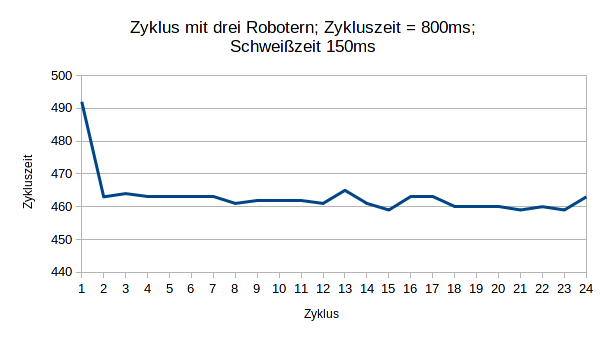
\includegraphics[width=\linewidth]{../evaluation_results/3_800.png}
  \caption{Durchlauf mit drei Robotern und \newline 800ms Zykluszeit}
  \label{fig:eval_3_800}
 \end{subfigure}
 \begin{subfigure}{.5\textwidth}
  \centering
  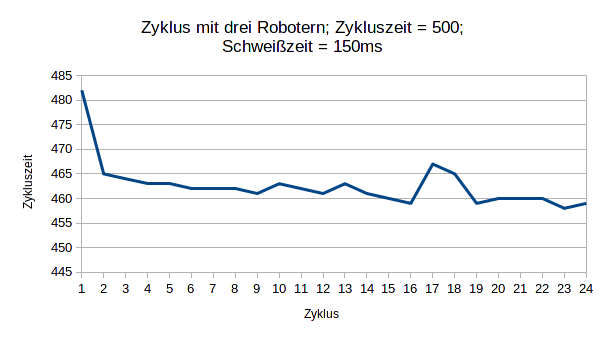
\includegraphics[width=\linewidth]{../evaluation_results/3_500.png}
  \caption{Durchlauf mit drei Robotern und \newline 500ms Zykluszeit}
  \label{fig:eval_3_500}
 \end{subfigure}
 \caption{Experimentdurchlauf mit drei Robotern}
 \label{fig:eval_3}
\end{figure}

Im ersten Durchlauf \ref{fig:eval_3} mit jeweils 800ms \ref{fig:eval_3_800} und 500ms \ref{fig:eval_3_500}
Zykluszeit ist zu erkennen, dass der erste Zyklus länger braucht als die darauf folgenden. Dies liegt daran,
dass am Anfang durch die Registrierung der Roboter und der Wahl des ersten Koordinators mehr Nachrichten
verarbeitet werden müssen als später im Durchlauf. Die Zykluszeit pendelt sich nach dem ersten Zyklus bei
einem Durchschnittswert von 461ms ein. Wenn man die Schweißzeit pro Roboter rausrechnet (150ms pro Roboter,
also 450ms pro Zyklus) kommt man auf 11ms reine Bearbeitungszeit des Algorithmus.

\clearpage

\subsection{Experimentdurchlauf mit vier Robotern}
\label{lamport_problem}

\begin{figure}[h]
 \begin{subfigure}{.5\textwidth}
  \centering
  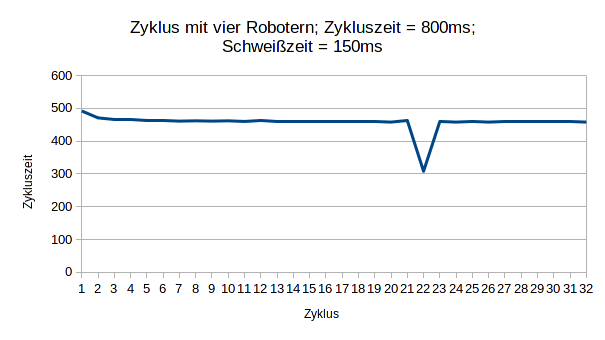
\includegraphics[width=\linewidth]{../evaluation_results/4_800.png}
  \caption{Durchlauf mit vier Robotern und \newline 800ms Zykluszeit}
  \label{fig:eval_4_800}
 \end{subfigure}
 \begin{subfigure}{.5\textwidth}
  \centering
  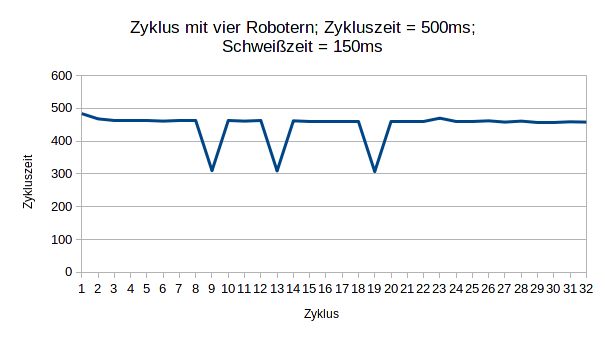
\includegraphics[width=\linewidth]{../evaluation_results/4_500.png}
  \caption{Durchlauf mit vier Robotern und \newline 500ms Zykluszeit}
  \label{fig:eval_4_500}
 \end{subfigure}
 \caption{Experimentdurchlauf mit vier Robotern}
 \label{fig:eval_4}
\end{figure}

Ein Experimentdurchlauf mit vier Robotern \ref{fig:eval_4} unterscheidet sich nicht von einem mit drei Robotern
hinsichtlich Zykluszeiten. Eine Auffälligkeit existiert jedoch in Form von auffällig kurzen Zykluszeiten (siehe
Zyklus 22 in \ref{fig:eval_4_800} oder Zyklus 9, 13 und 20 in \ref{fig:eval_4_500}. Dies ist darauf zurückzuführen,
dass alle Roboter gleichzeitig versuchen per Lamport Zugriff auf die Ressource zu erhalten. Wenn nun ein ein 
Prozess bei allen anderen den Zugriff erbittet und niemand in der Zeit selbst einen Zugriff auf die Ressource
erbittet, greift er auf die Ressource zu, obwohl ein anderer Prozess mit höherer ID und gleichem
Timestamp eher Zugriff auf die Ressource erhalten würde. Lamport erwartet allerdings eine klare Reihenfolge der
Events die in dem System auftreten \citep{lamport} (Erbitten der Ressource, Freigabe der Ressource).

\clearpage

\subsection{Auswirkung der Skalierung auf Zykluszeit}

\begin{figure}[h]
 \begin{subfigure}{.5\textwidth}
  \centering
  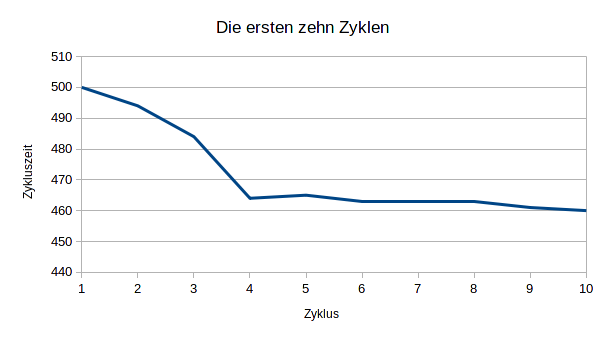
\includegraphics[width=\linewidth]{../evaluation_results/8_500_first10.png}
  \caption{Die ersten 10 Zyklen eines Durchlaufs mit 8 Robotern und 500ms Zykluszeit}
  \label{fig:eval_8_first10}
 \end{subfigure}
 \begin{subfigure}{.5\textwidth}
  \centering
  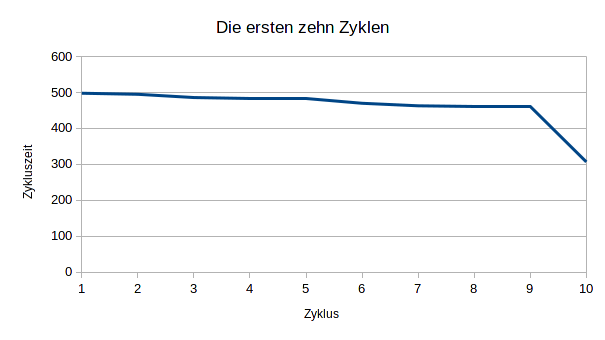
\includegraphics[width=\linewidth]{../evaluation_results/16_500_first10.png}
  \caption{Die ersten 10 Zyklen eines Durchlaufs mit 16 Robotern und 500ms Zykluszeit}
  \label{fig:eval_16_first10}
 \end{subfigure}
 \caption{Experimentdurchlauf mit 8 und 16 Robotern}
 \label{fig:eval_8_16_first10}
\end{figure}

In \ref{fig:eval_8_16_first10} zu erkennen hat die unterschiedliche Problemgröße der Durchläufe einen Einfluss
auf die Zykluszeiten am Anfang des Experiments. Während bei 8 Robotern die Zykluszeit bereits ab dem 4. Zyklus
(\ref{fig:eval_8_first10}) sich auf dem Durchschnittswert von 461ms einpendelt braucht es bei 16 Robotern
10 Zyklen (\ref{fig:eval_16_first10}). Die mit jedem zusätzlich teilnehmenden Roboter steigende
Nachrichtenkomplexität sorgt für diese anfangs höheren Zykluszeiten. Es melden sich mehr Roboter im System an
demnach steigt auch die Zahl der Registrierungsnachrichten.


% Fazit
% @author Tristan Ropers
%
\chapter{Fazit}

Die Umsetzung des Lamort Algorithmus für gegenseitigen Ausschluss in verteilten Systemen war erfolgreich.
Mit der in dieser Arbeit beschriebenen Lösung ließ sich der Algorithmus in eine selbst entwickelte
RPC-Lösung integrieren und am beschriebenen Use-Case demonstrieren. Die in Kapitel \ref{requirements}
entwickelten Anforderungen konnten umgesetzt werden, sowie die Design-Goals eines verteilten Systems
\citep{tanenbaumvansteen} insofern sie nicht durch den Rahmen der Aufgabenstellung bereits eingeschränkt
wurden (siehe \ref{requirements}). Eine Ausnahme stellt das in Kapitel \ref{lamport_problem} erläuterte
Fehlverhalten der hier erarbeiteten Lösung dar.


%\bibliographystyle{plain}
\bibliographystyle{dinat}
\bibliography{literature}

% Appendix
\appendix
% !TEX root = ../thesis.tex
% appendix example chapter
% @author Thomas Lehmann
%
\chapter{Anhang}


\IGlossary

\Istatement

\end{document}
